\section{Formalizace problému}

Problém má dva hráče:

\begin{itemize}
    \item agenta,
    \item protivníka.
\end{itemize}

Agent má k dispozici pohybové akce:

\begin{itemize}
    \item nahoru,
    \item dolů,
    \item doleva a
    \item doprava.
\end{itemize}

Na druhé straně protivník na začátku \bf{rozestavuje bandity} a poté, pokud hráč spustí alarm, může \bf{jednoho banditu přemístit} z označeného místa na místo jiné.

Strategie agenta se skládá ze sekvence jednotlivých povolených pohybů a strategie protivníka pouze z výběru úvodního rozestavení a v případě alarmu změny pozice jednoho agenta.

Informační sety budou ve hře dvě:

\begin{enumerate} 
    \item vytvořené uzly na začátku hry po rozmístění banditů,
    \item pokud dojde k alarmu, tak jednotlivé možnosti, jak změnit rozestavení banditů.
\end{enumerate}

\section{Herní strom}

\begin{center}
    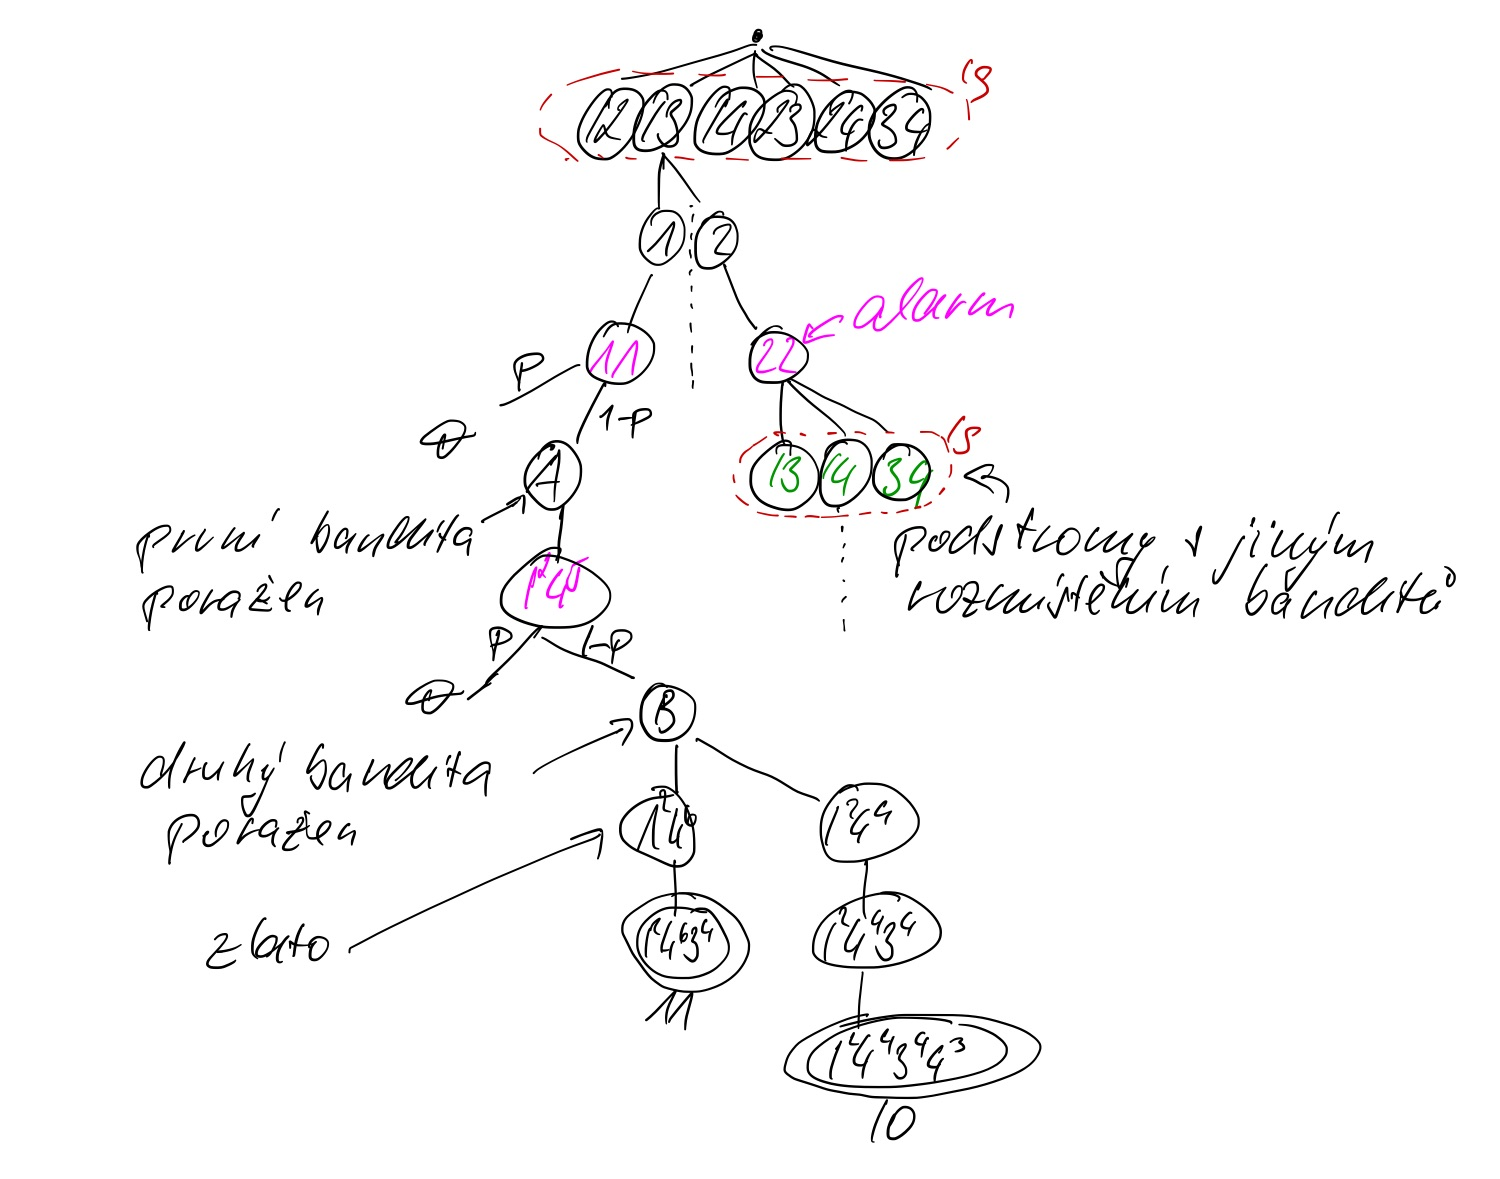
\includegraphics[width=\textwidth]{herni-strom}
\end{center}

\bf{Vysvětlivky}
\begin{itemize}
    \item První informační set jsou jednotlivá úvodní rozmístění banditů.
    \item Fialovou barvou textu je označen příchod na nebezpečné místo.
    \item Uzly agenta jsou označeny pomocí čísel, kde 1 = Up, 2 = Left, 3 = Down, 4 = Right. Tedy kombinace 12 znamená, že se agent nejdříve posunul o jedno pole nahoru a poté o jedno pole doleva.
    \item Zelenou barvou jsou označeny uzly s novým rozmístěním banditů po spuštění alarmu. Čísla 1 - 4 označují jednotlivá nebezpečná místa, přičemž v herním stromě agent stojí na nebezpečném místě s pořadovým číslem 2.
\end{itemize}

\section{Závěr}

Úlohu jsem z hlediska náročnosti velice podcenil a proto není hotový generátor lineárního programu pro zadanou úlohu.
